\documentclass[11pt,a4paper]{article}
\usepackage[margin=2.3cm]{geometry}
\usepackage[T1]{fontenc}
\usepackage{lmodern}
\usepackage{amsmath,amssymb}
\usepackage{enumitem}
\usepackage{microtype}
\usepackage{fancyhdr}
\usepackage{tikz}
\usetikzlibrary{arrows.meta,automata,positioning}
\usepackage[hidelinks]{hyperref}
\setlength{\parindent}{0pt}
\setlength{\parskip}{6pt}
\setlength{\headheight}{14pt}
\setlist[enumerate]{itemsep=4pt,topsep=3pt}
\pagestyle{fancy}
\fancyhf{}
\fancyhead[L]{CSCI 3130 --- Homework 4 Solutions}
\fancyhead[R]{\thepage}
\newcommand{\emptystr}{\lambda}
\newcommand{\derive}{\Rightarrow}
\newcommand{\derivestar}{\Rightarrow^{*}}

\begin{document}
\begin{center}
  {\Large\bfseries Formal Languages and Automata Theory}\\[3pt]
  {\large\bfseries Homework 4 --- Solutions}
\end{center}
Throughout, $\lambda$ denotes the empty string.

\section*{Q1. Removing undesirable productions (20\%)}
The given grammar is
\[
\begin{aligned}
S&\to aaA\mid aBB, & A&\to aA\mid\lambda,\\
B&\to bB\mid bbC, & C&\to B.
\end{aligned}
\]

\textbf{Step 1: Remove $\lambda$-productions.}
The only nullable variable is $A$. Omitting $A$ from $S\to aaA$ and
$A\to aA$ introduces $S\to aa$ and $A\to a$, respectively.
After deleting $A\to\lambda$, we obtain
\[
\begin{aligned}
S&\to aaA\mid aa\mid aBB, & A&\to aA\mid a,\\
B&\to bB\mid bbC, & C&\to B.
\end{aligned}
\]
There is no need to preserve a start-symbol $\lambda$-production, since
the original grammar cannot generate $\lambda$.

\textbf{Step 2: Remove unit-productions.}
The only unit-production is $C\to B$. Replace it by the non-unit
productions of $B$:
\[
\begin{aligned}
S&\to aaA\mid aa\mid aBB, & A&\to aA\mid a,\\
B&\to bB\mid bbC, & C&\to bB\mid bbC.
\end{aligned}
\]

\textbf{Step 3: Remove useless productions.}
Both $A$ and $S$ are generating variables: $A\derive a$ and $S\derive aa$.
Neither $B$ nor $C$ is generating. Every production with left side $B$
or $C$ leaves a $B$ or $C$ on the right, so a derivation starting with
either variable can never become a terminal string.
Delete $B,C$ and every production involving them, including $S\to aBB$.
The remaining variables $S,A$ are both reachable from $S$.

Thus an equivalent grammar with no unit-, useless-, or
$\lambda$-productions is
\[
\boxed{\begin{aligned}
S&\to aaA\mid aa,\\
A&\to aA\mid a.
\end{aligned}}
\]

\textbf{Language generated.}
In the original grammar, $A$ generates $a^{*}$, and the branch
$S\to aBB$ never yields a terminal string. Hence
\[
\boxed{L(G)=\{a^{n}:n\ge 2\}.}
\]
The new grammar generates $aa$ directly, and generates $a^n$ for each
$n\ge3$ using $S\derive aaA\derivestar aa\,a^{n-2}$; it generates no other strings.

\newpage
\section*{Q2. Conversion to Chomsky normal form (30\%)}
The original grammar is
\[
\begin{aligned}
S&\to AB\mid a,\\
A&\to aAB\mid b,\\
B&\to bB\mid bAC,\\
C&\to c.
\end{aligned}
\]

\textbf{Step 1: Check preliminary simplifications.}
There are no $\lambda$-productions or unit-productions.
All variables are generating: $A\derive b$, $C\derive c$,
$B\derive bAC\derivestar bbc$, and $S\derive a$.
All are reachable: $S\to AB$ reaches $A,B$, and $B\to bAC$ reaches $C$.
Thus no useless productions need to be removed.
Also, $S$ never occurs on a right-hand side, so no new start symbol is needed.

\textbf{Step 2: Replace terminals in right-hand sides of length at least two.}
Introduce fresh variables
\[
T_a\to a,\qquad T_b\to b.
\]
Keep the existing single-terminal productions unchanged. The grammar becomes
\[
\begin{aligned}
S&\to AB\mid a,\\
A&\to T_aAB\mid b,\\
B&\to T_bB\mid T_bAC,\\
C&\to c,\\
T_a&\to a,\\
T_b&\to b.
\end{aligned}
\]
No variable $T_c$ is necessary, since $c$ occurs only in $C\to c$.

\textbf{Step 3: Binarize the length-three right-hand sides.}
Introduce fresh variables
\[
D\to AB,\qquad E\to AC.
\]
Replace $A\to T_aAB$ by $A\to T_aD$, and replace $B\to T_bAC$
by $B\to T_bE$. The final grammar is
\[
\boxed{\begin{aligned}
S&\to AB\mid a,\\
A&\to T_aD\mid b,\\
B&\to T_bB\mid T_bE,\\
C&\to c,\\
D&\to AB,\\
E&\to AC,\\
T_a&\to a,\\
T_b&\to b.
\end{aligned}}
\]

\textbf{Verification.}
Every production now has the form $X\to YZ$ (two variables) or
$X\to t$ (one terminal). Hence the grammar is in CNF.
The new variables simply abbreviate fixed substrings of the original
right-hand sides; for example,
$A\derive T_aD\derive aD\derive aAB$ and
$B\derive T_bE\derive bE\derive bAC$.
Expanding or contracting these abbreviations preserves the language.

\newpage
\section*{Q3. Determinism of the PDAs (20\%)}
A PDA is deterministic if both of the following conditions hold:
\begin{enumerate}[label=(\roman*)]
  \item For every state $q$, stack-top symbol $X$, and
  $x\in\Sigma\cup\{\lambda\}$, the set $\delta(q,x,X)$ has at most one element.
  \item For every fixed pair $(q,X)$, if $\delta(q,\lambda,X)$ is nonempty,
  then $\delta(q,x,X)$ is empty for every input symbol $x\in\Sigma$.
\end{enumerate}
The second condition prevents a choice between consuming an input symbol
and taking a $\lambda$-transition from the same configuration.
As stated in the question, all unlisted transitions are empty.

\subsection*{1. Deterministic}
The transitions are
\[
\delta(q_0,a,z)=\{(q_0,Az)\},\qquad
\delta(q_0,\lambda,A)=\{(q_1,\lambda)\}.
\]
Each transition set is a singleton. Moreover, the two transitions require
\emph{different stack-top symbols}:
\begin{itemize}
  \item With top $z$, the only possible move reads $a$.
  \item With top $A$, the only possible move is the $\lambda$-move to $q_1$.
\end{itemize}
Thus no fixed pair $(q,X)$ admits both an input-consuming move and a
$\lambda$-move. Both determinism conditions hold.
\[
\boxed{\text{PDA 1 is deterministic.}}
\]

\subsection*{2. Nondeterministic}
The transitions are
\[
\delta(q_0,a,z)=\{(q_0,Az)\},\qquad
\delta(q_0,\lambda,z)=\{(q_1,z)\}.
\]
Although both transition sets are singletons, they apply to the same
state and stack top, $(q_0,z)$. If the next unread symbol is $a$, two
moves are enabled:
\[
(q_0,aw,z\beta)\vdash(q_0,w,Az\beta)
\quad\text{or}\quad
(q_0,aw,z\beta)\vdash(q_1,aw,z\beta).
\]
Here $w$ is the remaining input after that $a$, and $\beta$ is the stack
suffix below $z$ (possibly empty).
This violates condition (ii).
\[
\boxed{\text{PDA 2 is nondeterministic.}}
\]

\newpage
\section*{Q4. NPDA for $L=\{a^ncb^n:n\ge0\}$ (30\%)}
\textbf{Idea.}
Push one $A$ for each $a$ before the unique $c$, then pop one $A$ for
each $b$ after $c$. Enter the final state when the stack has returned
to its bottom marker. Acceptance requires that the entire input has been read.

\textbf{Formal construction.}
Let
\[
M=(Q,\Sigma,\Gamma,\delta,q_0,Z_0,F),
\]
where $Q=\{q_0,q_1,q_f\}$, $\Sigma=\{a,b,c\}$,
$\Gamma=\{A,Z_0\}$, and $F=\{q_f\}$.
The initial stack consists of $Z_0$; the leftmost stack symbol is the top.
The nonempty transitions are
\[
\begin{aligned}
\delta(q_0,a,Z_0)&=\{(q_0,AZ_0)\}, &
\delta(q_0,a,A)&=\{(q_0,AA)\},\\
\delta(q_0,c,Z_0)&=\{(q_1,Z_0)\}, &
\delta(q_0,c,A)&=\{(q_1,A)\},\\
\delta(q_1,b,A)&=\{(q_1,\lambda)\}, &
\delta(q_1,\lambda,Z_0)&=\{(q_f,Z_0)\}.
\end{aligned}
\]
All unlisted transitions are empty. The state $q_f$ has no outgoing transitions.

\textbf{State transition diagram.}
An edge label $x,X\to\gamma$ means: read $x$ (read nothing if
$x=\lambda$), pop $X$, and replace it by $\gamma$.
\begin{center}
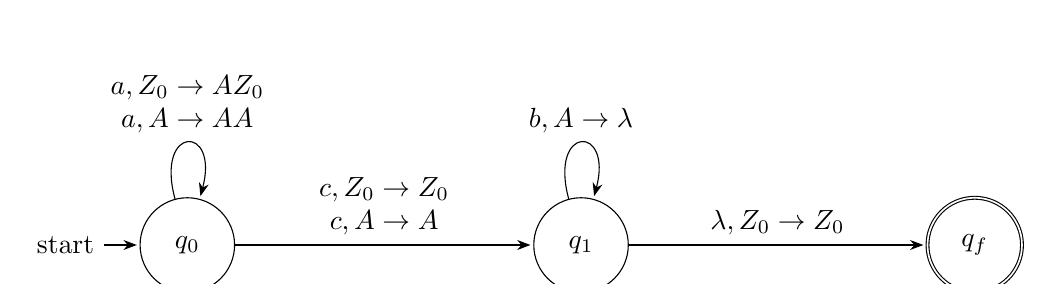
\begin{tikzpicture}[
  >=Stealth,shorten >=1pt,node distance=5.0cm,on grid,auto,
  every state/.style={minimum size=12mm},
  every edge/.style={draw,->},
  initial text={start}
]
  \node[state,initial] (q0) {$q_0$};
  \node[state,right=of q0] (q1) {$q_1$};
  \node[state,accepting,right=of q1] (qf) {$q_f$};
  \path
    (q0) edge[loop above] node[align=center]
      {$a,Z_0\to AZ_0$\\$a,A\to AA$} (q0)
    (q0) edge node[align=center]
      {$c,Z_0\to Z_0$\\$c,A\to A$} (q1)
    (q1) edge[loop above] node {$b,A\to\lambda$} (q1)
    (q1) edge node {$\lambda,Z_0\to Z_0$} (qf);
\end{tikzpicture}
\end{center}

\textbf{Correctness.}
For every $n\ge0$, the machine has the accepting computation
\[
\begin{aligned}
(q_0,a^ncb^n,Z_0)
&\vdash^{*}(q_0,cb^n,A^nZ_0)\\
&\vdash(q_1,b^n,A^nZ_0)\\
&\vdash^{*}(q_1,\lambda,Z_0)
\vdash(q_f,\lambda,Z_0).
\end{aligned}
\]
In particular, $n=0$ gives
$(q_0,c,Z_0)\vdash(q_1,\lambda,Z_0)\vdash(q_f,\lambda,Z_0)$,
so $c$ is accepted.

Conversely, any accepting computation must pass from $q_0$ to $q_1$
by reading exactly one $c$. Before this transition, only $a$'s can be read,
each pushing one $A$. After it, only $b$'s can be read, each popping one
$A$. The final-state transition is possible only when all those $A$'s
have been popped. Since acceptance also requires empty remaining input,
the number of $b$'s equals the number of $a$'s. Hence the accepted string
is exactly $a^ncb^n$ for some $n\ge0$, proving $L(M)=L$.

\end{document}
